% -- frame 1---
\begin{frame}{Set up the testing machine}
\begin{itemize}
    \item Ubuntu 20.04
    \item CPU Intel Xeon X5647
    \item 8 GB RAM
    \item 1 Gbps
    \item Kubernetes 1.20.7 and 1.23.0
    \item OpenFaaS 0.21.1
    \item 1 master node
    \item Calico as CNI
    \item Longhorn for persistent volumes
    \item Docker Engine as CRI \pause \textit{\alert{dockershim is no longer supported after 1.24}}
    
\end{itemize}
    
\end{frame}

% -- frame 2--
\begin{frame}{Choose the testing functions}
Let's choose 14 tests from the FunctionBench serverless benchmarking suite [4].

\begin{itemize}
    \item 8 from CPU \& Memory category.
    \item 4 from Disk I/O category.
    \item 2 from Network performance category.
\end{itemize}
    
\end{frame}

% --- frame 3 ---
\begin{frame}{How do we run?}

5 tests for each Kubernetes distribution. Executed using the recommended OpenFaaS of-watchdog template for Python 3.7.

\pause

We'll see performances for:

\begin{itemize}
    \item Cold start
    \item Serial execution
    \item Parallel execution using a single replica
    \item Parallel execution using native OpenFaaS auto scaling
    \item Parallel execution using Kubernetes HPA
\end{itemize}

\end{frame}

% -- frame 4 --
\begin{frame}{Cold start performance}
Each function is executed 100 times to test the cold start delay. \pause
After every execution, the number of instances for the function is scaled to 0. A new container instance needs to be created before a response is returned.
\end{frame}

% -- frame 5 --
\begin{frame}{Cold start performance — Results}
Kubespray exhibits a 15\% increase compared to both K3s and MicroK8s.

\begin{figure}
    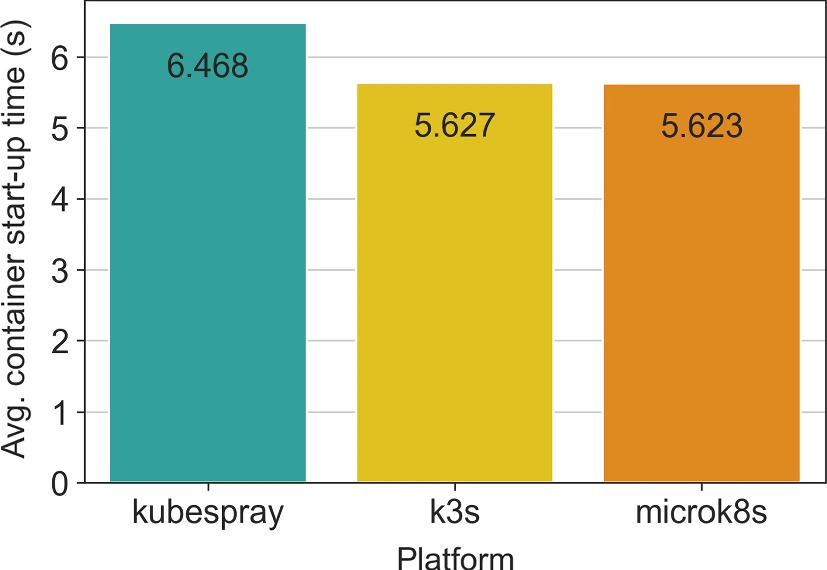
\includegraphics[width=0.5\linewidth]{static/11227_2022_4430_Fig1_HTML.jpg}\hfill
    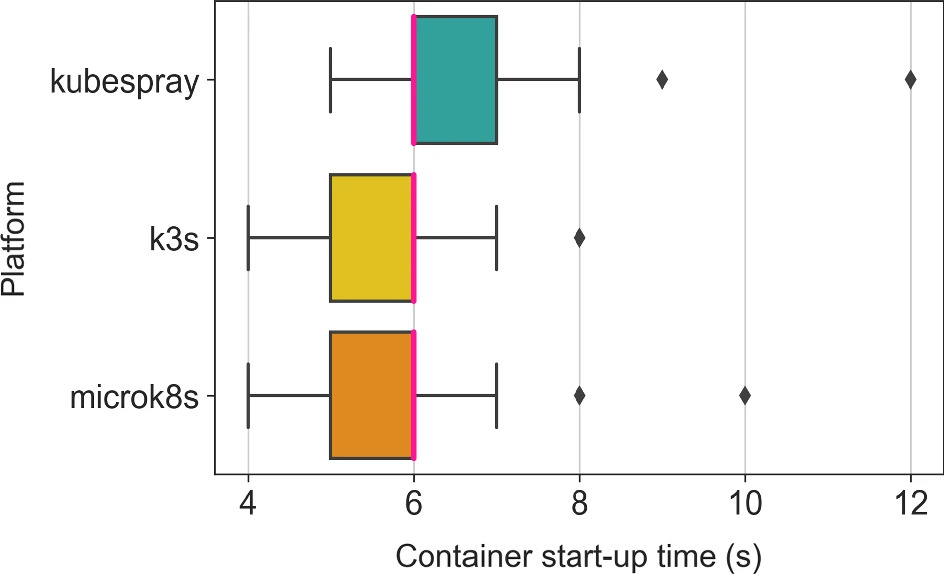
\includegraphics[width=0.5\linewidth]{static/11227_2022_4430_Fig2_HTML.jpg}
\end{figure}

\end{frame}

% -- frame 6 --
\begin{frame}{Cold start performance — Results}
Is the performance difference between K3s and MicroK8s statistically significant?
\pause

Using a Mann-Whitney \(U\) test with \(\alpha = 0.05\) and 
\begin{itemize}
    \item H0: the two populations are equal
    \item H1: the two populations are not equal
\end{itemize}

we have a \(p\)-value \(= 0.202 > 0.05\), so we can't reject the null hypothesis.

\end{frame}

% -- frame 7 --
\begin{frame}{Serial execution performance}
Each function is continuously invoked for a period of 5 min using a single thread. Once a response is received, a new request is immediately sent. Auto-scaling is manually disabled.
\end{frame}

% -- frame 8 --
\begin{frame}{Serial execution performance — Results}
Once again, Kubespray results are slower than both K3s and MicroK8s.

\begin{figure}
    \centering
    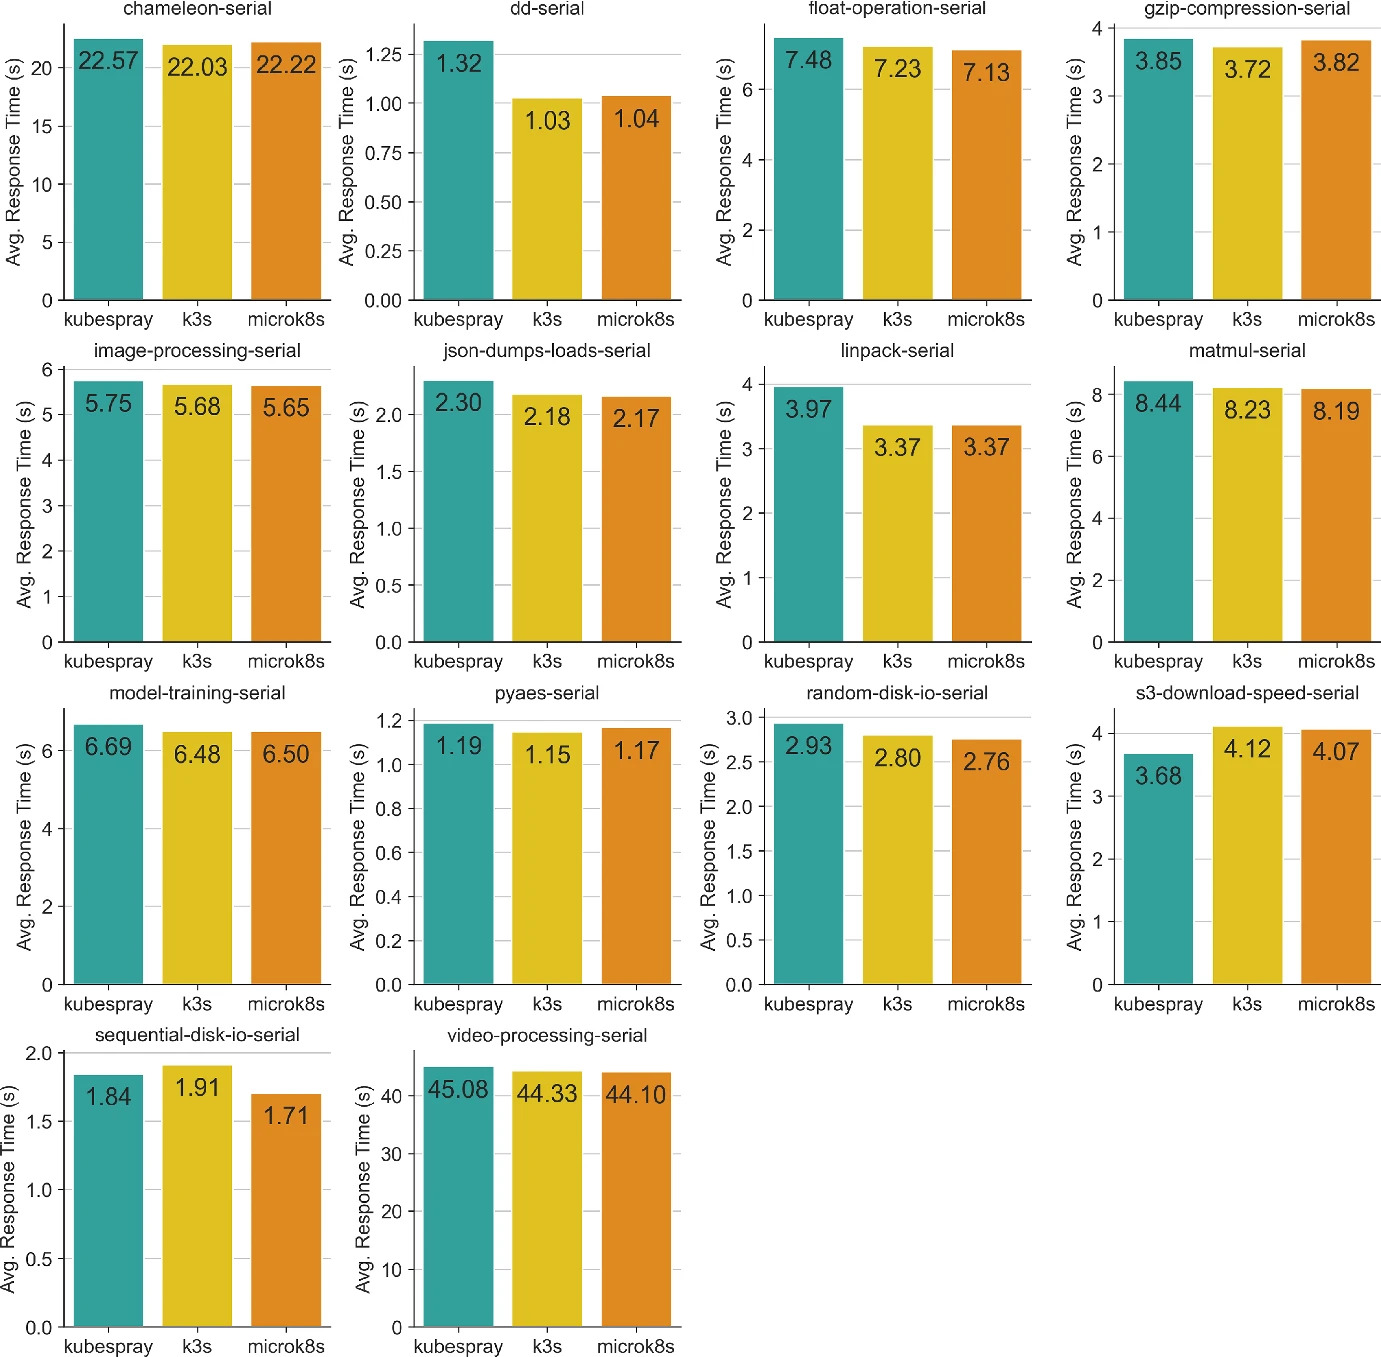
\includegraphics[width=0.6\linewidth]{static/11227_2022_4430_Fig5_HTML.jpg}
\end{figure}
\end{frame}

% -- frame 9 --
\begin{frame}{Serial execution performance — Results}
How can I compare these three results?
\pause

Using a Kruskal-Wallis test with \(\alpha = 0.05\) and 
\begin{itemize}
    \item H0: the population medians are equal
    \item H1: the population medians are not equal
\end{itemize}

where the null hypothesis failed to be rejected for the video-processing test. \pause
\\ Keeping the same hypothesis we can perform the Mann-Whitney \(U\) test for both K3s and MicroK8s and, this time, the null hypothesis is rejected in 10 of the 14 tests. The null hypothesis can't be rejected for 3 CPU and 1 network benchmarks.
\end{frame}

% -- frame 10 --
\begin{frame}{Parallel execution performance using a single replica}
Each function is invoked for a fixed amount of time using varying concurrency to determine the performance of the auto-scaling behavior. \textit{Reduced isolation.}
\end{frame}


% -- frame 11 --
\begin{frame}{Parallel execution performance using a single replica — Results}
This time Kubespray has better performance than both K3s and MicroK8s for 6 of the 14 tests.

\begin{figure}
    \centering
    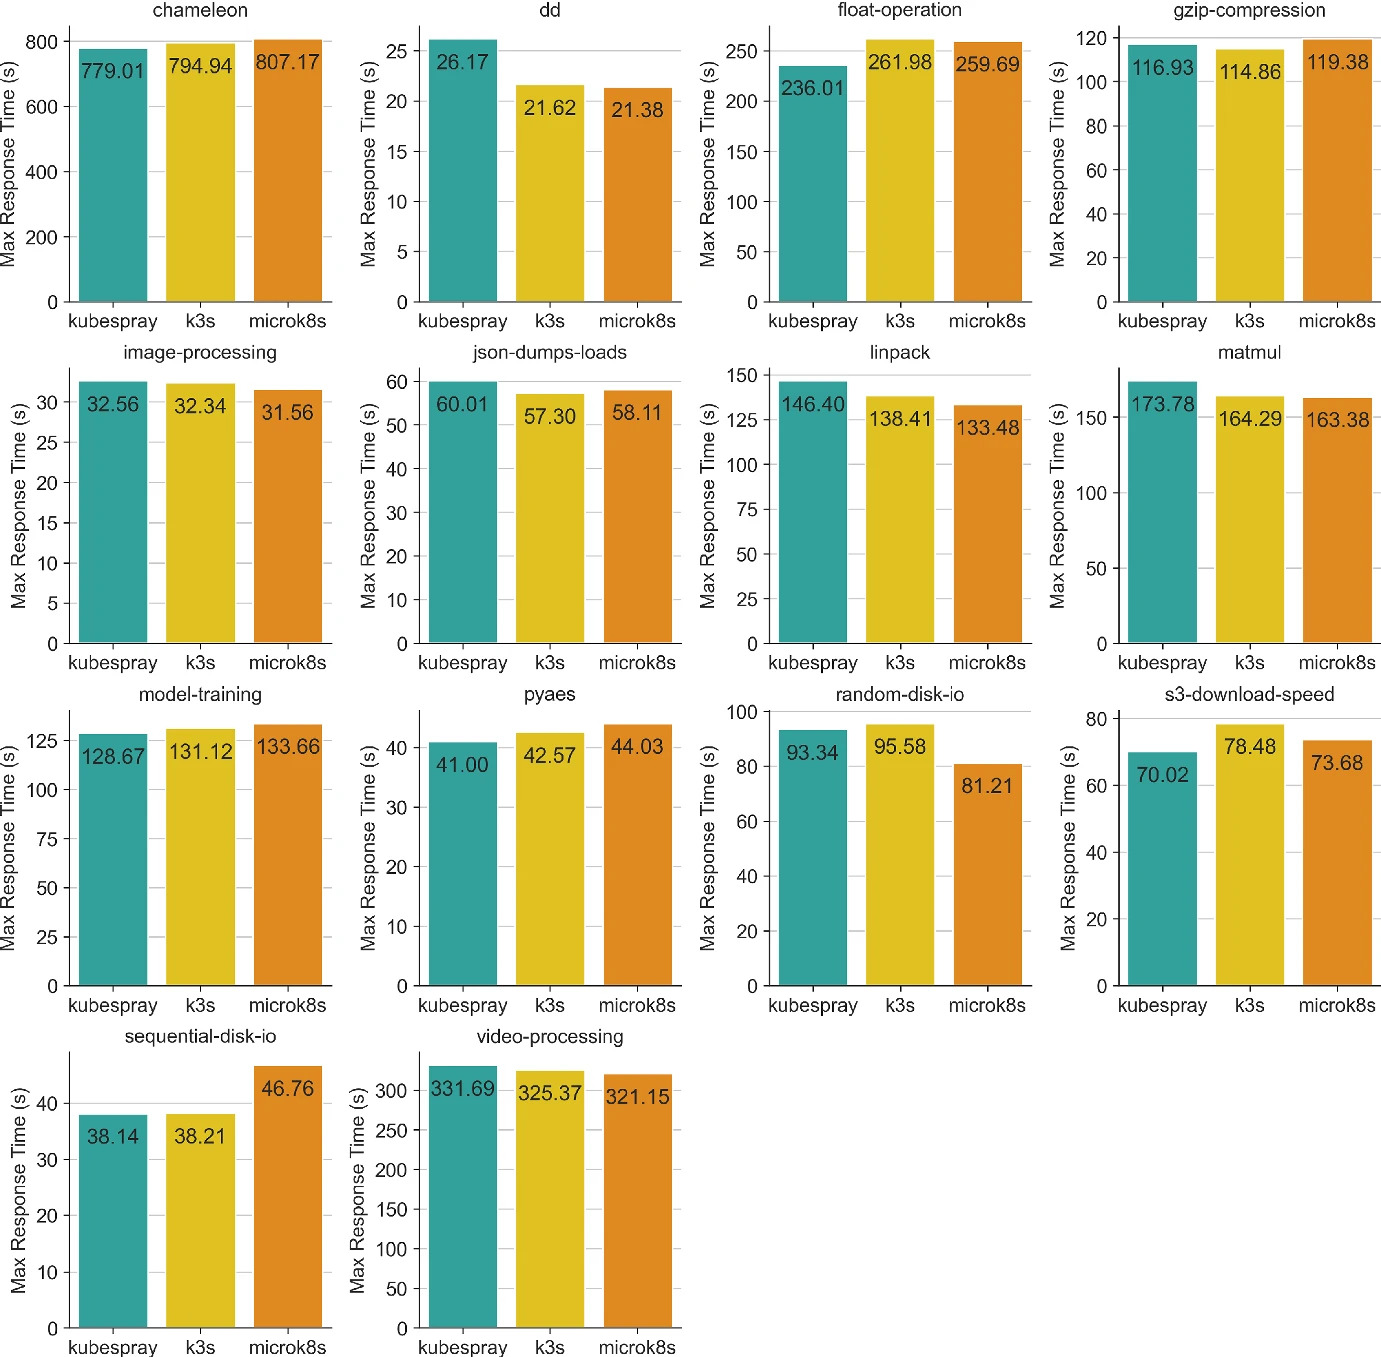
\includegraphics[width=0.5\linewidth]{static/11227_2022_4430_Fig6_HTML.jpg}
\end{figure}
\end{frame}

% -- frame 12 --
\begin{frame}{Parallel execution using native OpenFaaS auto scaling}
Each function is invoked for a fixed amount of time using varying concurrency to determine the performance of the auto-scaling behavior.
\pause
\\
It tests the number of successful invocations per second for the last 10 seconds: if the number is larger than 5, it scales up the number of function instances up to a preconfigured maximum.
\end{frame}


% -- frame 13 --
\begin{frame}{Parallel execution using native OpenFaaS auto scaling  — Results}
Performances are tests by 1 req/s from 6 concurrent workers for more than 200s, successfully reaching the defined threshold for the maximum number of replicas.\\
The current number of deployed replicas are not taken but this leads to suboptimal scaling decision scaling to maximum number of configured replicas or not scaling at all under a consistent load.
\end{frame}


% -- frame 14 --
\begin{frame}{Parallel execution using Kubernetes Horizonal Pod Autoscaler}
Each function is invoked as the same way as the previous test using the Kubernetes native mechanism. For this test, HPA is configured with a profile which is fired whenever the float-operation function has used more than 350 CPU shares (0.35 of a core). \pause
We find out results for three different execution strategy:

\begin{itemize}
    \item Start from 1 replica, execute 2 concurrent req/s, increasing the concurrency rate by 2 every 5 min, until 48 req/s are achieved.
    \item Start from 1 replica, execute 40 concurrent req/s, decreasing the concurrency rate by 2 every 5 min, until 2 req/s are achieved.
    \item Start from 1 replica and vary the number of concurrent requests every 5 min using the strategy 8, 1, 20, 4, 40, 24, 1, 4, 16, 1, 36, 32.
\end{itemize}
\end{frame}


% -- frame 15 --
\begin{frame}{Parallel execution using Kubernetes Horizonal Pod Autoscaler  — Results}
Kubespray exhibits higher response times across the three tests, while the results obtained from K3sand MicroK8s are similar.

\begin{figure}
    \centering
    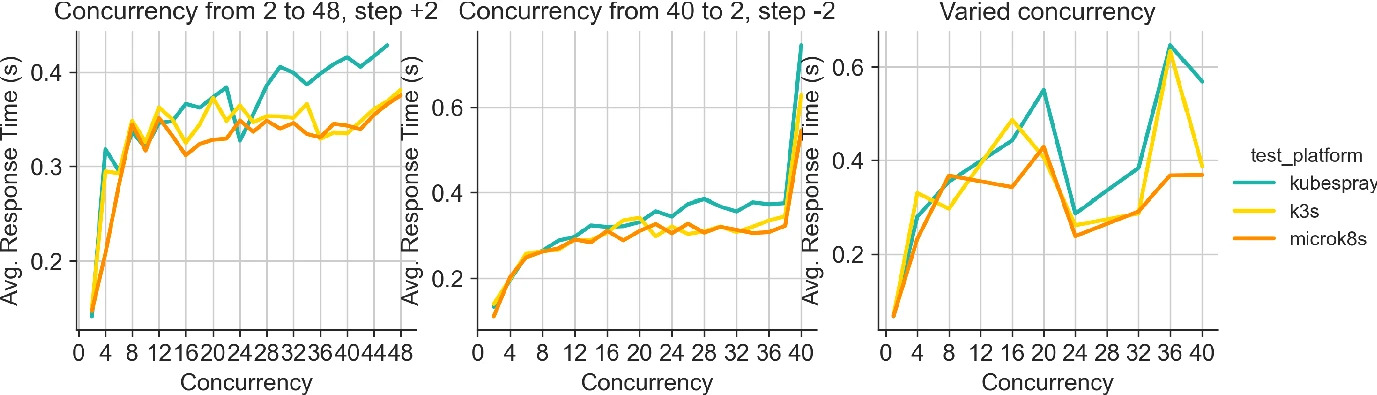
\includegraphics[width=1\linewidth]{static/11227_2022_4430_Fig8_HTML.jpg}
\end{figure}
\end{frame}
